\chapter{Экспериментальная часть}

В данном разделе сравним работу каждого алгоритма.

\section{Временные характеристики}

Сравним матричный алгоритм поиска расстояния Левенштейна и Дамерау-Левенштейна.
Для сравнения возьмем строки длиной [10, 20, 30, 50, 100, 200]. 
Так как подсчет расстояния считается короткой задачей, воспользуемся усреднением массового эксперимента. 
Для этого сложим результат работы алгоритма n раз (n >= 10), после чего поделим на n. 
Тем самым получим достаточно точные характеристики времени. 
Сравнение произведем при n = 500.
Результат можно увидеть на рис. \ref{fg:ref4}. При короткой длине разница по времени минимальна, при увеличении длины строки алгоритм поиска расстояния Левенштейна с небольшим опережением вырывается вперед. Это обосновывается тем, что у алгоритма поиска расстояния Дамерау-Левенштейна задействуется еще одна операция, которая замедляет алгоритм.

\begin{figure}[ht!]
	\centering{
		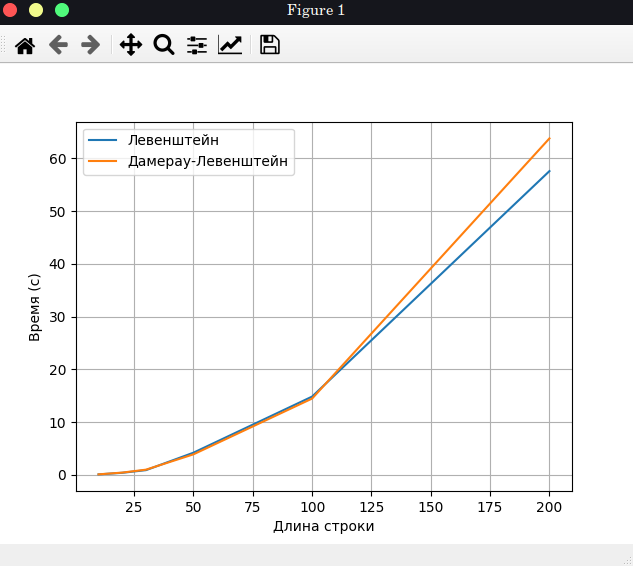
\includegraphics[width=0.6\textwidth]{img/graphLev-LevDam.png}
		\caption{Сравнение времени работы алгоритма поиска расстояния Левенштейна и Дамерау-Левенштейна}
		\label{fg:ref4}}
\end{figure}

Далее проведем сравнительный анализ временных характеристик рекурсивной и матричной реализаций алгоритма Левенштейна. 
Возьмем строки длиной [2, 3, 5, 7, 8], n положим равным 50.
Результат можно увидеть на рис. \ref{fg:ref5}.
Такая большая разница во времени объясняется тем, что в рекурсивном алгоритме Левенштейна много рекурсивных вызовов с однотипными параметрами.

\begin{figure}[ht!]
	\centering{
		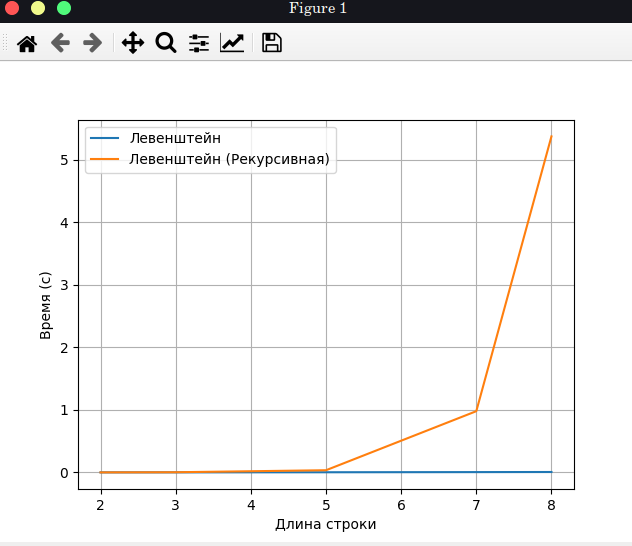
\includegraphics[width=0.6\textwidth]{img/graphLev-LevRec.png}
		\caption{Сравнение времени работы рекурсивной и матричной реализаций алгоритма Левенштейна.}
		\label{fg:ref5}}
\end{figure}

\section{Характеристики по памяти}

На рисунке \ref{fg:ref6} представлено дерево вызовов рекурсивного алгоритма Левенштейна.
Видно, что на третьем уровне встречаются повторные вызовы. 
Чем больше будет уровень, тем чаще будут вызываться функции с однотипными аргументами, что может привести к превышению максимальной глубины рекурсии. 
При строках длиной 2 подпрограмма вызовется 18 раз. 
Каждый вызов задействует 32 мегабайт (замеры проведены с помощью  библиотеки memory\_profiler \cite{bib6}).
В итоге нам потребуется 576 мегабайт для рекурсивных вызовов, в то время, когда в матричном алгоритме используется 42 мегабайта. 

\begin{figure}[ht!]
	\centering{
		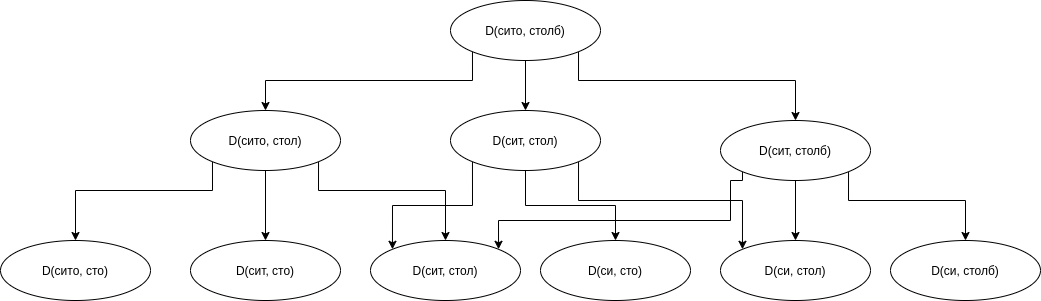
\includegraphics[width=0.8\textwidth]{img/rec_example.png}
		\caption{Сравнение времени работы рекурсивной и матричной реализаций алгоритма Левенштейна.}
		\label{fg:ref6}}
\end{figure}

\section{Сравнительный анализ алгоритмов}

Приведенные характеристики показывают нам, что рекурсивная реализация алгоритма очень сильно проигрывает по времени и по памяти.\\
Во время печати очень часто возникают ошибки связанные с транспозицией букв, поэтому алгоритм поиска расстояния Дамерау-Левенштейна предпочтительнее, не смотря на то, что он проигрывает по времени алгоритму Левенштейна.\\
По аналогии с первым абзацем можно сделать вывод о том, что рекуррентный алгоритм поиска расстояния Дамерау-Левенштейна будет более затратный, как по памяти, так и по времени по сравнению с матричной реализацией алгоритма поиска расстояния Дамерау-Левенштейна.

\section{Вывод}

В данном разделе было произведено сравнение количества затраченного времени и памяти вышеизложенных алгоритмов.
Самым быстрым оказался матричный алгоритм нахождения расстояния Левенштейна.


